\documentclass{article}
\usepackage[margin=2cm,bottom=2cm]{geometry}
\usepackage{hyperref}
\usepackage{comment}
\usepackage[utf8]{inputenc}
\usepackage{graphicx}
\usepackage{mathtools}
\graphicspath{ {bootstrapping.png} }

\newcommand\tab[1][1cm]{\hspace*{#1}}

\begin{document}
\title{COMP/CMPE 314 - Principles of Programming Languages - Notes}
\author{Chris Stephenson, Istanbul Bilgi University, Department of Mathematics, and course students}
\maketitle


\section*{Answers of the quiz \#1}
\subsection*{Question \#1}
\subsubsection*{Language}
  \begin{itemize}
        \item A finite alphabet
        \item A set of strings of the symbols in the alphabet (usually infinitive)
   \end{itemize}
 
\subsubsection*{Grammar}
  \begin{itemize}
   \item A set of productions (rewriting rules)
   \item A finite alphabet of terminal symbols
   \item A finite set of non-terminal symbols
   \item A sentence symbol ( S )
  \end{itemize}

Simple language: [a] 
  \begin{itemize}
   \item $S \rightarrow a$
   \item $S \rightarrow aS$ (infinite)
   
   $S \rightarrow number$\newline
   $S \rightarrow S + S$\newline
   $S \rightarrow S * S$\newline
   $S \rightarrow (S)$\newline
   alphabet = [+, *, (), number]
  
  \end{itemize}
  

\subsection*{Question \#2}

  \begin{verbatim}
    (define (interp [a : ArithC]) : number
        (type-case ArithC a
            [numC (n) n]
            [plusC (l r) (+ (numC-n l) (numC-n r))]
            [multC (l r) (* (numC-n l) (numC-n r))]))
  \end{verbatim}
  
  \begin{verbatim}
    In this code;
    (+ 4 3) works but,
    (+ (* 3 7) (+ 4 2)) crashes
  \end{verbatim}
  
  In order to make it work we need to change numC to interp like this

  \begin{verbatim}
    (define (interp [a : ArithC]) : number
        (type-case ArithC a
            [numC (n) n]
            [plusC (l r) (+ (interp l) (interp r))]
            [multC (l r) (* (interp l) (interp r))]))
  \end{verbatim}
  
  
\section*{Programming Languages}
\begin{tabular}{c c}
 \textbf{Programming Languages} & \textbf{Kinds of Programming Languages}\\
 \begin{tabular}{ l c r }
    Java & Assembly & Swift \\
    Python & C & Prolog \\
    Ruby & C\# & Fortran \\
    Objective-C & Racket & R \\
    Lisp & Haskell & Whitespace \\
    Javascript & Pascal & Giuseppe \\
    Scala & HTML & Ada \\
    Pick & Perl & XML \\
    SQL & BASH & XSDL \\
    Scratch &  &  \\
  \end{tabular}
  &
  \begin{tabular}{ c }
    Markup Language \\
    Functional \\
    Object oriented \\
    Procedural \\
    Scripting \\
    Graphical \\
    Experimental \\
    Declarative \\
    Machine \\
  \end{tabular}
\end{tabular}


\begin{flushleft}
The code below is valid in Java and also valid in C. \\
What value does the function/method \verb|funny2| returns?

\begin{verbatim}
 int funny(int a, int b){
    return a + 2 * b;
 }
 
 int funny2(){
    int a = 2;
    return funny(a++, a++);
 }
\end{verbatim}

In this example the value returned in Java and C are different. Java returns 8 but C returns 7.\\
This situation caused by the compilers of this languages. In \verb|funny(a++, a++)| statement Java starts from left \verb|a++| but C starts from right \verb|a++|.\linebreak

Let us consider this now\\
1000000 + 2000000\\
"1000000" + "2000000"\\
In the first example Java returns a negative integer value. Because it assigns numbers default by int and maximum int value is 2,147,483,647.\\
In the second one Java concatenates the two strings like "10000002000000" (But some languages adds them)\linebreak

All programming languages are data formats for data input to other programs.\\
\begin{figure}[h]
  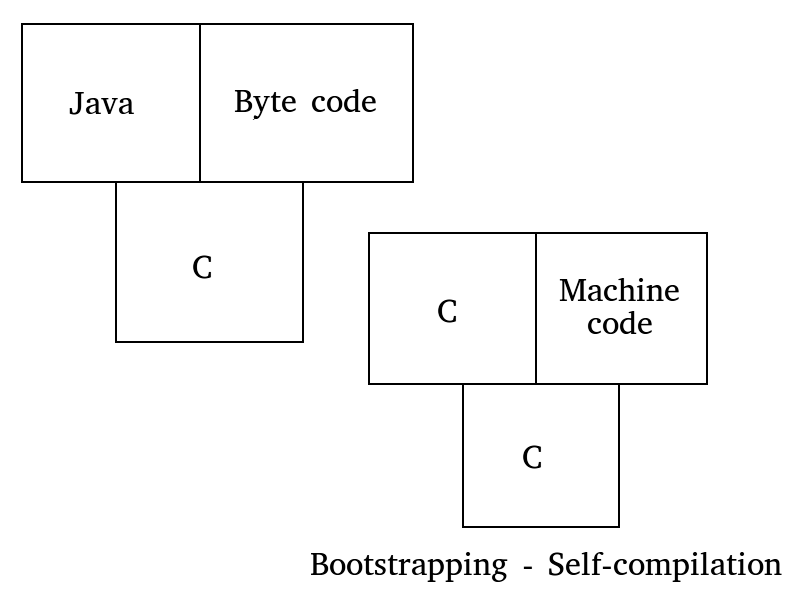
\includegraphics[scale=0.2]{bootstrapping}
\end{figure}

\center{Program text $\xrightarrow{parse}$ Data Structure $\xrightarrow{interp/eval}$ Answer}\\
\begin{verbatim}
 (eval (parse '(+ 2 (* 3 4))))
\end{verbatim}
Parsing is common to all compilers/interpreters


\end{flushleft}





\end{document}